\chapter{Debugging support}

\begin{quote}
  \textit{Debugging is twice as hard as writing the code in the first place. Therefore, if you write the code as cleverly as possible, you are, by definition, not smart enough to debug it.}\begin{flushright}
    \tiny{Brian W. Kernighan}
  \end{flushright}
\end{quote}

We already mentioned in first chapter that to debug programs in high level programming languages we need the compiler to emit debugging information.
But debugging support must also be provided by operating system (if there is one) and by processor itself.
In this chapter, we discuss how debugging is supported at various levels.

\section{Instruction set architecture}
In first chapter it was said that CPU can only execute machine code which is made of instructions
and that it has certain registers. Which instructions and registers the CPU has can differ from CPU to CPU.
This is specified by \textit{Instruction Set Architecture} (ISA) \cite{aps-isa}. It is an abstract interface between
the hardware and lowest level software (machine code). It contains all information needed to write a program in machine
code. In general, ISA specifies following:
\begin{itemize}
    \item Set of machine code instructions - Specifies instructions the ISA has and what operands each instruction has.
    \item Register set - Which registers the ISA has\footnote{Strictly speaking ISA doesn't have to use registers. It's possible to use only stack or accumulator, but most used ISAs use registers. }.
    \item Addressing modes - Possible methods to refer to memory or register.
\end{itemize}
There are other specification, they are not relevant to this thesis. For each instruction and operand there is
specified how they should be encoded into binary (remember, that's what the CPU can understand).
CPU then \textit{implements} some ISA. If two different CPUs implements the same ISA then they should be able to run the same machine code program.
For example, most PC use the \textit{x86} architecture \cite{aps-isa}, althrough the \textit{ARM} architecture is on the rise with the Apple sillicon.

The x86 architecture is so called \textit{Complex Instruction Set Architecture} (CISC). It contains many instructions that do
many things at once, have varying length and takes multiple clock cycles to complete \cite{intel-manual}. On the other hand
the ARM architecture is \textit{Reduced Instruction Set Architecture} (RISC). The number of instructions is smaller, they
are intended to be small building blocks from which complex operations may be created by using many of them. Each instruction in RISC also
has same length. Both architectures have their pros and cons, althrough some literature suggest that in modern days the choice of architecture
is irrelevant if one is only considering performance and power consuption  \cite{riscvscisc1, riscvscisc2}.
Unless specified otherwise the rest of this chapter will be talking about x86.

In first chapter we briefly mentioned that machine code programs can instead be written in Assembly language.
Assembly is almost 1:1 mapping to machine code. When showing programs, we will instead use Assembly. In figure
\ref{fig:assembly-example2}, we present another example of a program that was compiled from C to Assembly of the x86 architecture.
As seen, instructions have various operands. Most often registers (\texttt{RBP, RSP, EAX}), memory (\texttt{[rbp-4]} is reference to memory at address which
is in register \texttt{rbp} minus $4$), or labels (like \texttt{L2}). Labels are not part of machine code, instead
memory address has to be provided. This is a small part where assembly and machine code differ.
For detailed overview of the x86 instructions see \cite{intel-manual}.

\begin{figure}\label{fig:assembly-example2}
    \begin{lstlisting}
max:
    push    rbp
    mov     rbp, rsp
    mov     QWORD PTR [rbp-24], rdi
    mov     DWORD PTR [rbp-28], esi
    mov     rax, QWORD PTR [rbp-24]
    mov     eax, DWORD PTR [rax]
    mov     DWORD PTR [rbp-4], eax
    mov     DWORD PTR [rbp-8], 1
    jmp     .L2
.L3:
    mov     eax, DWORD PTR [rbp-8]
    cdqe
    lea     rdx, [0+rax*4]
    mov     rax, QWORD PTR [rbp-24]
    add     rax, rdx
    mov     eax, DWORD PTR [rax]
    cmp     DWORD PTR [rbp-4], eax
    cmovge  eax, DWORD PTR [rbp-4]
    mov     DWORD PTR [rbp-4], eax
    add     DWORD PTR [rbp-8], 1
.L2:
    mov     eax, DWORD PTR [rbp-8]
    cmp     eax, DWORD PTR [rbp-28]
    jl      .L3
    mov     eax, DWORD PTR [rbp-4]
    pop     rbp
    ret
    \end{lstlisting}
    \caption{Compiled C program with GCC 9.4 compiler as x86 assembly.}
\end{figure}

\subsection{Registers}

The x86 architecture has a set of general purpose registers.
Some of these are
\begin{itemize}
    \item RAX - Accumulator for operands and results data,
    \item RCX - Counter for string and loop operations,
    \item RSP - Stack pointer,
    \item RBP - Pointer to data on the stack.
\end{itemize}
The names and number of general purpose registers change based on bit mode. 64-bit mode has 16 of them, while 32-bit has 8.
Althrough the \texttt{RSP} and \texttt{RBP} are called general purpose they are often only used for pointing at the top of the stack,
resp. to the base of the stack. Stack is special part of program memory, it mostly has LIFO semantics.
It can be used to store intermediate result, arguments to functions, return address etc.
This register is weird in a sense that it has this very special purpose but is still considered part of
the general purpose registers. One might use it for storing calculations, but it would make
rest of the instructions that work with stack behave unexpectedly \cite{intel-manual}.

Instruction pointer register (RIP) contains address of the current instruction to be executed.
As we mentioned in Introduction \todo{ref}, programs are executed sequentially from top to bottom,
with certain instructions having the ability to change the control flow. When an instruction get
executed, the size of the instruction will be added to the value in RIP register. This will advance
the instruction pointer to the next instruction. Or, if the instruction changes control flow,
the value in instruction pointer will be changed to the destination of the instruction.

Another interesting register is the \texttt{EFLAGS} register. The register contains group
of flags, which can alter various behavior of the CPU, or the CPU itself sets them
as result of some instruction. For example the instruction \texttt{cmp} compares its two operands
and if they are the same the \textit{zero} flag in the \texttt{EFLAGS} register will be set.

\subsection{Interrupts}
Interrupt is a special request to the CPU to stop execution of current program and to quickly react to
the reason that caused the request \cite{aps-interrupts}. Example of such event can be keyboard press or error in an program (division by zero).
There are two main categories \cite{intel-manual}
\begin{itemize}
    \item An \textbf{interrupt} is an asynchronous\footnote{Meaning that the interrupt may happen when another instruction is being processed (not on the CPU clock edge).} event that is typically triggered by an Input/Output (IO) device.
    \item An \textbf{exception}\footnote{Unfortunately, this term will become quite overloaded in this thesis.} is a synchronous event that is generated when the processor detects one or more
          predefined conditions when executing an instruction. These are further divided into three classes: faults, traps and aborts.
\end{itemize}
When an interrupt or exception happens, the processor halts execution of current program and switches to specific interrupt handler.
Example of an exception is the \texttt{INT3} instruction. When this instruction is executed an interrupt is generated.
This instruction is specifically meant to be used as a breakpoint. So, we have a way of how the CPU
can stop execution and handle the breakpoint.


\section{Debugging native programs}
For now, we pretended that source-level debuggers can magically work with lines of source code. However, for programs to be run they first need to be compiled to native code - a series of binary instructions (there are also interpreted programs, which we will touch upon later). The debugger then interacts with this native code. It, by itself, has no idea that line $x$ corresponds to address $y$. The compiler must embed this information in the executable, or somewhere else, for the debugger to know this type of information. One of such standards of encoding debug information is DWARF format \cite{dwarf}, which will be thoroughly described in \todo{TODO} section. 

As we mentioned, some debuggers only work on the assembly level. They do not perform any mapping to the source code. And the debuggers that do have to work with machine code all the same. In the next section, we will explore how assembly-level debuggers are implemented. The implementation itself can greatly differ based on the operating system or target machine. The following section aims to describe the most often used OS and targets.

\subsection{Breakpoints}
Term \textit{debuggee} means a program that is being debugged. The instuction architecture \textit{x86} contains special instruction \mintinline{c}{INT3}, opcode \mintinline{c}{0xCC}. When processor executes this instruction it issues special interrupt and advances program counter by one. The interrupt is then handled by OS. How the handling is done depends heavily on OS and will be covered later.

Consider the following code \todo{Typeset these guys correctly}
\begin{minted}{asm}
0x0 xor    eax,eax        33 c0
0x2 mov    esp,ebp        8b e5
0x4 pop    ebp            5d
\end{minted}
To create a breakpoint on address \mintinline{c}{0x02}, the debugger needs to replace the code on that location with the \mintinline{c}{0xCC}. The result would look like this:
\begin{minted}{asm}
0x0 xor    eax,eax        33 c0
0x2 int3                  cc e5
0x4 pop    ebp            5d
\end{minted}
The processor executes the \mintinline{c}{xor}, then the \mintinline{c}{int3}, this sends the interrupt, but because that instruction was executed the program counter is now set to \mintinline{c}{0x3}. If the debugger would just told the program to continue it would execute the instruction at that point, which begins with \mintinline{c}{0xe5}. If the replaced instruction is one byte in size, it would skip the replaced instruction and execute the rest of the program. If it was bigger, it would essentially interpret the body of that instruction as new instruction. This would most likely cause a crash. The debugger needs to deal with this. 

\subsection{Trap flags}
The x86 architecture contains special \textit{Trap flag}. When it is set, the processor issues interrupt \mintinline{c}{INT1} every time an instruction is executed. \todo{Doplnit nebo smazat: Viz konzultace}.

\subsection{ptrace}
Linux offers special system call which is very handy for debugging. It is called \mintinline{c}{ptrace} \cite{ptrace} - process trace. It has following signature: \mintinline{c}{ptrace(PTRACE_COMMAND, pid, ...)}. It takes a \mintinline{c}{PTRACE_COMMAND}, which specifies the behaviour of the function (for example \mintinline{c}{PTRACE_SINGLESTEP} for single step), pid of some process and some other parameters, depending on the \mintinline{c}{PTRACE_COMMAND}. 

It allows to observe and control the execution of another process, which will most often be the debuggee. When the debugee is traced, it will stop each time a signal is delivered\footnote{\mintinline{c}{SIGKILL} is an exception, it will have its usual effect.}. The debugger will be notified at its next call to \mintinline{c}{waitpid}. This system call return value will indicate the reason debuggee stopped. \mintinline{c}{ptrace(PTRACE_TRACEME, ...)} called from a child of the debugger will cause the debugger to \textit{attach} to the child, which is the debuggee. The debugger can then issue other commands to the child. There are also \mintinline{c}{PTRACE_ATTACH} and \mintinline{c}{PTRACE_SEIZE}, which can be used for attaching to existing process.

\mintinline{c}{ptrace} has many commands, here are some of the most important:
\begin{itemize}
    \item \mintinline{c}{PTRACE_PEEKTEXT, PTRACE_PEEKDATA} - Read tracee's memory,
    \item \mintinline{c}{PTRACE_POKETEXT, PTRACE_POKEDATA} - Write into tracee's memory,
    \item \mintinline{c}{PTRACE_GETREGS} - Read tracee's register values,
    \item \mintinline{c}{PTRACE_SETREGSET} - Modify tracee's register values,
    \item \mintinline{c}{PTRACE_GETSIGINFO} - Retrieve information about the signal that caused tracee to stop,
    \item \mintinline{c}{PTRACE_CONT} - Restart the stopped tracee process,
    \item \mintinline{c}{PTRACE_SINGLESTEP} - Restart the stopped tracee but stop it after executing one instruction.
\end{itemize}

\todo{Describe how they are used in real code}

\subsection{Windows}
Windows also has built-in support for debugging at the Win32API layer \cite{windows-msdn-debugging-api, windows-press-debugging-api}.
It builds on \textit{debug events} and \textit{debug functions}. Summary of some of the functions that Win32 API offers which all help with debugging:

\begin{itemize}
    \item \mintinline{c}{DebugActiveProcess} - Attaches the debugger to an active process.
    \item \mintinline{c}{DebugBreakProcess} - Causes a breakpoint exception to occur in the specified process. 
                                          This passes control of the process to the debugger if there is one.
    \item \mintinline{c}{WaitForDebugEvent} - Waits for new debug events.
    \item \mintinline{c}{ContinueDebugEvent} - Continue the process execution after processing debug event.
    \item \mintinline{c}{OutputDebugString} - Sends a string to the debugger for display.
    \item \mintinline{c}{ReadProcessMemory} and \mintinline{c}{WriteProcessMemory} - Read and modify process virtual address space.
    \item \mintinline{c}{FlushInstructionCache} - Flushes instruction cache of the process.
\end{itemize}

The general structure of Windows debugger can be seen in figure \ref{fig:win32debugger}.
The debugger waits for debug events via function \mintinline{c}{WaitForDebugEvent}.
This function has a timeout parameter, so the debugger can also do other things while it's waiting.
These events are put in a queue, so the debugger will not miss any.

\begin{figure}
    \centering
    \scalebox{0.8}{
    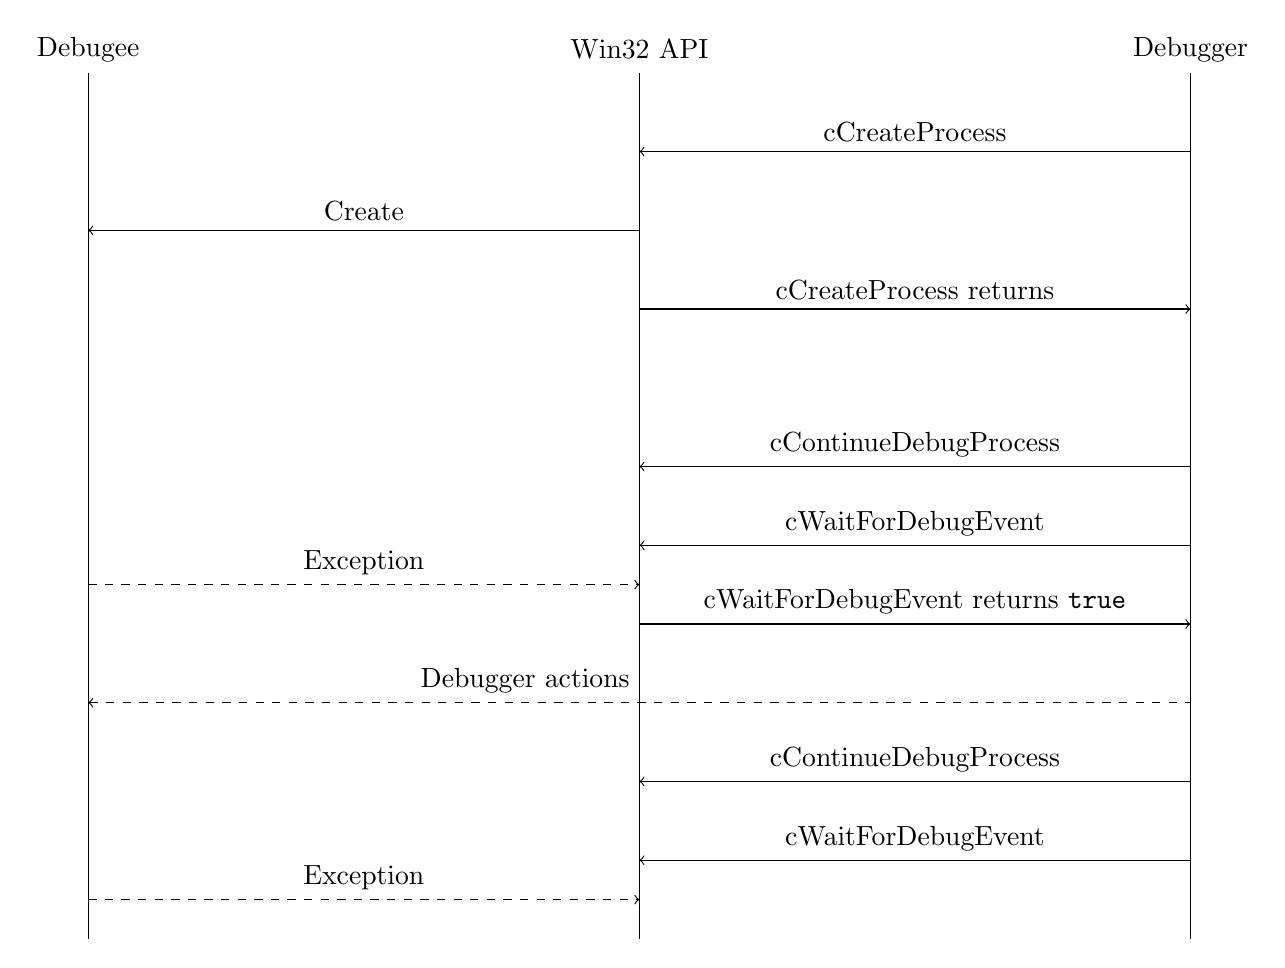
\begin{tikzpicture}
        \draw (-7,0) -- (-7,-11) (0,0) -- (0,-11) (7,0) -- (7,-11);
        \node at (-7,.3) {Debugee};
        \node at (0,.3) {Win32 API};
        \node at (7,.3) {Debugger};
        \draw[<-] (0,-1) -- node[midway,above] {\mintinline{c}{CreateProcess}} (7,-1);
        \draw[<-] (-7,-2) -- node[midway,above] {Create} (0,-2);
        \draw[->] (0,-3) -- node[midway,above] {\mintinline{c}{CreateProcess} returns} (7,-3);
        \draw[<-] (0,-5) -- node[midway,above] {\mintinline{c}{ContinueDebugProcess}} (7,-5);
        \draw[<-] (0,-6) -- node[midway,above] {\mintinline{c}{WaitForDebugEvent}} (7,-6);
        \draw[dashed,->] (-7,-6.5) -- node[midway,above] {Exception} (0,-6.5);
        \draw[->] (0,-7) -- node[midway,above] {\mintinline{c}{WaitForDebugEvent} returns \texttt{true}} (7,-7);
        \draw[dashed, <-] (-7, -8) -- node[above left] {Debugger actions} (7, -8);
        \draw[<-] (0,-9) -- node[midway,above] {\mintinline{c}{ContinueDebugProcess}} (7,-9);
        \draw[<-] (0,-10) -- node[midway,above] {\mintinline{c}{WaitForDebugEvent}} (7,-10);
        \draw[dashed,->] (-7,-10.5) -- node[midway,above] {Exception} (0,-10.5);
    \end{tikzpicture}
    }
    \caption{A sequence diagram for debugger using Windows api. Inspired by \todo{NI-REV 6. lecture}}
    \label{fig:win32debugger}
\end{figure}

The debug events are thoroughly described in subsection \ref{section:Debug Events}. The main point of interest is the exceptions.
By these, we do not mean the standard C++ exceptions but rather Microsoft \textit{Structured Exception Handling}.

\subsubsection*{Debug Events}\label{section:Debug Events}
Debugging events are various incidents in the debuggee that causes the system to notify the debugger \cite{windows-msdn-debug-events}. These are stored in special \mintinline{c}{DEBUG_EVENT} structure, which is received in \texttt{WaitForDebugEvent} call from debugger. This structure contains various information about the event, the internals can be seen on figure \ref{fig:DebugEvent}. These events include loading and unloading a DLL, creating and exiting a process, sending debug strings via the \mintinline{c}{OutputDebugString} and so on. It also includes exceptions, those are probably the most important for us. 
\begin{figure}
\begin{minted}{c}
typedef struct _DEBUG_EVENT {
  DWORD dwDebugEventCode;
  DWORD dwProcessId;
  DWORD dwThreadId;
  union {
    EXCEPTION_DEBUG_INFO      Exception;
    CREATE_THREAD_DEBUG_INFO  CreateThread;
    CREATE_PROCESS_DEBUG_INFO CreateProcessInfo;
    EXIT_THREAD_DEBUG_INFO    ExitThread;
    EXIT_PROCESS_DEBUG_INFO   ExitProcess;
    LOAD_DLL_DEBUG_INFO       LoadDll;
    UNLOAD_DLL_DEBUG_INFO     UnloadDll;
    OUTPUT_DEBUG_STRING_INFO  DebugString;
    RIP_INFO                  RipInfo;
  } u;
} DEBUG_EVENT, *LPDEBUG_EVENT;
\end{minted}
\caption{Structure which contains info about debug event.}
\label{fig:DebugEvent}
\end{figure}

\subsubsection*{Structured Exception Handling}
This feature is specific to Windows only. For example, if division by zero was performed in a program on Linux,
a signal would be sent to the process. Windows don't have signals, instead, it uses Structured Exception Handling \cite{windows-msdn-seh}. 
From now on, we will be using the abbreviation 'SEH'.
An exception is an event that requires execution of code outside the normal flow of control. There are software exceptions,
like throwing an exception explicitly or by OS, and hardware exceptions, like the division by zero we mentioned.
Instruction with opcode \mintinline{c}{0xCC}, which is used for breakpoints, will also raise an exception. SEH unifies both of these things into one.

When an exception is triggered, control is transferred to the system. It saves the state of the thread and some other information.
This information can be used to continue execution from the point where the exception was thrown when it is resolved. It also
contains information about which type of exception was thrown, if execution can continue after handling the exception, address where the
exception occured and some others\footnote{See MSDN documentation \cite{windows-msdn-seh} for full detailed list}.
The system then searches for an exception handler which will handle the exception. The search is performed in this order:

\begin{enumerate}
    \item If the process is debugged the debugger is notified.
    \item If it is not or the debugger does not handle the exception, the frame-based exception handler is to be found\footnote{The handlers are not very important to us, see MSDN documentation if you're interested \cite{windows-msdn-seh}.}
    \item If no frame-based handler can be found, or no handler handles the exception, but the process is being debugged then the debugger gets notified once again.
    \item The system provides default handling, which is to terminate the program via \mintinline{c}{ExitProcess} most of the time.
\end{enumerate}

Here we see that every exception that occurs in the debuggee causes the debugger to be notified. Breakpoints are also caused by an exception, as was briefly mentioned before. There are two possible notifications to the debugger. The first is known as \textit{first-chance} notification \cite{windows-msdn-dbg-exc-handling}. The debugger can (and should) inspect the information about the exception and see if it was a breakpoint or single-step. These only occurs if the process is debugged (it wouldn't happen otherwise) and the debugger should handle them. If it is something else it can ignore the exceptions. When the program is continued via \mintinline{c}{ContinueDebugEvent}\footnote{This function has a special parameter, which is used to tell that the exception was or was not handled.}, the debugger is notified once again if no appropriate exception handler was found for the exception. This is known as \textit{last-chance} notification because if the debugger does not handle the exception the debuggee will be terminated. It gives the user a chance to debug why is his process terminating.

Here are some exceptions that tie into debugging:
\begin{itemize}
    \item \mintinline{c}{STATUS_BREAKPOINT} - Raised when a hardware-defined breakpoint was encountered. This includes the mentioned \mintinline{c}{INT3} instruction.
    \item \mintinline{c}{STATUS_SINGLE_STEP} - Raised when a single step was completed, ie. when instruction was executed and the trap flag is set.
\end{itemize}

\subsubsection*{Tying it all together}
Now we have all necessary building block to build a simple proof of concept Windows debugger. On figure \ref{fig:windows-debugger-mainloop}, you can see a basic idea of a main loop of the debugger. It waits for debug events and branches depending of the type of event. It needs not only handle exceptions, but other events also. For example if the debugee creates a thread that is something the debugger should be aware of. Modern debuggers trace all threads of the program.

\todo{Pridat dalsi figure kde je jak se hanndlujou tyhle blbosti} However, exceptions are the most interesting for us. There, breakpoint and single step handling should be done. On both of these, the debugger should handle the exception itself, so this is the \textit{first chance} notifications. There is also an \mintinline{DBG_CONTROL_C}, which happens on CTRL + C keyboard press. This should terminate the program. The debugger will pass the first chance and catch the last chance exception, so user has a final chance to look at the program state before it exits.

\begin{figure}
    \begin{minted}{c}
void EnterDebugLoop(const LPDEBUG_EVENT DebugEv)
{
   DWORD dwContinueStatus = DBG_CONTINUE; // exception continuation
   for(;;)
   {
      WaitForDebugEvent(DebugEv, INFINITE);
      switch (DebugEv->dwDebugEventCode)
      {
         case EXCEPTION_DEBUG_EVENT:
            // Handle exception debug events
         // Other debug events
      }
   ContinueDebugEvent(DebugEv->dwProcessId,
                      DebugEv->dwThreadId,
                      dwContinueStatus);
   }
}
\end{minted}
\caption{Windows debugger main loop}
\label{fig:windows-debugger-mainloop}
\end{figure}

\section{Compiler support}
\todo{Moved from introduction here for the time being}
When we talked about evolution of programming from machine code to assembly to higher level languages, we haven't
talked about how they are executed. Machine code can be directly executed by processor, as we said, it is a sequence
of binary. Assembly is text, processors don't understand text. But assembly can be mapped to machine code almost 
1:1\footnote{There are some exceptions, like labels. But translating them is not very difficult.}.

However, high level programming languages do not map 1:1 to assembly. Some are close to it, like C, while others
are miles away, like Haskell. But as was said, processors understand only machine code. To this end, programs that
can translate source code into machine code, were created. They are called compilers and the translation process is
called compiling. For example, for the C language one might use the GCC or Clang compilers.
On figure \ref{fig:compiler-structure} can be seen basic structure of a compiler \cite{dragon-book}. 

\tikzstyle{compilerblock} = [rectangle, draw, minimum width=6cm, minimum height=1cm] 
\tikzstyle{tables} = [rectangle, draw, minimum width=4cm, minimum height=1cm] 
\begin{figure}\label{fig:compiler-structure}
    {\centering
    \begin{tikzpicture}
    \node (lexer)[compilerblock]{Lexical analyzer};
    \node (syntax)[compilerblock,below=of lexer]{Syntactic analyzer};
    \node (semantic)[compilerblock,below=of syntax]{Semantic analyzer};
    \node (imc)[compilerblock,below=of semantic]{Intermediate Code Generator};
    \node (gen)[compilerblock,below=of imc]{Code Generator};
    \node (symbol)[tables, left=of semantic]{Symbol table};
    \draw[->] (lexer) -- node[below] {} (syntax);
    \draw[->] (syntax) -- node[below] {} (semantic);
    \draw[->] (semantic) -- node[below] {} (imc);
    \draw[->] (imc) -- node[below] {} (gen);
    \end{tikzpicture} 
    \par}
    \caption{Simplified structure of a compiler. Some parts were left out, like optimizations.}
    \label{fig:compiler_tikz}
\end{figure}

\subsection{Lexical analyzer}
The lexical analyzer groups separate symbols into groups. For example the code
\begin{minted}{c}
foo = bar(1 + 2);
\end{minted}
might be translated into tokens like this
\begin{lstlisting}[stringstyle=\color{black}]
<id:"foo"> <assignment-operator> <id:"bar"> 
<left-bracket> <int-number:1> <plus-operator> 
<int-number:2> <right-bracket> <semicolon>
\end{lstlisting}
The Syntactic analyzer then works with these tokens.

\subsection{Syntantic and semantic analyzer}
Syntactic analysis accepts tokens and processes them into other intermediate representation. This is
most often an abstract syntax tree (abbr. AST, figure \ref{fig:ast}). It also checks that the source code complies to the grammar of the language.
Semantic analysis then checks that the program is semantically consistent. For example that used variable
has been declared before.

\begin{figure}\label{fig:ast}
    \centering
    \begin{tikzpicture}[,shorten >=1pt,node distance=1.8cm,on grid,initial/.style={}]
    \node (assignment) {$=$};
    \node (foo) [below left =of assignment] {id:foo};
    \node (bar) [below right =of assignment] {call:bar};
    \node (plus) [below right=of bar] {$+$};
    \node (one) [below left =of plus] {$1$};
    \node (two) [below right =of plus] {$2$};
    
    \draw[-, above, scale=0.7] 
    (assignment)   edge node[scale=0.7, left, yshift=0.1cm] {lhs}  (foo)
     (assignment)  edge node[scale=0.7, right, yshift=0.1cm] {rhs}  (bar)
     (bar)         edge node[scale=0.7, right, yshift=0.1cm] {expr} (plus)
     (plus)        edge node[scale=0.7, right, yshift=0.1cm] {rhs}  (two)
     (plus)        edge node[scale=0.7, left, yshift=0.1cm] {lhs}  (one);
    \end{tikzpicture}
    \caption{Simplified example of an abstract syntax tree.}
    \label{fig:astgraph}
\end{figure}
 
\subsection{Intermediate code generation}
This part converts AST into some other representation, most commonly called IR\footnote{IR means intermediate representation.
AST is also intermediate representation, but if we use IR we mean this one.}. IR is closer to machine code, to be easily translated,
but retain some properties that makes it easier to work with it. There are many types of IR. One of the most popular compilers, LLVM, uses
single static assignment (SSA) \cite{llvm}. Example of LLVM IR can be found on figure \ref{fig:llvm-ir-example}. Compilers perform most
optimizations on this intermediate representation. 

\begin{figure}\label{fig:llvm-ir-example}
    \begin{minted}{llvm}
        define dso_local i32 @_Z6squarei(i32 %0) {
          %2 = alloca i32, align 4
          store i32 %0, i32* %2, align 4
          %3 = load i32, i32* %2, align 4
          %4 = load i32, i32* %2, align 4
          %5 = mul nsw i32 %3, %4
          ret i32 %5
        }
    \end{minted}
    \caption{Simplified example of LLVM IR.}
\end{figure}

\subsection{Code generation}
Here, IR is translated directly to the target machine code or possibly assembly. Even though IR can seem very similar to assembly,
there are still some things to take care of. For example SSA IR doesn't have registers, it uses unlimited number of variables.
Other architectures might have some other traits that differ it from the IR and they all have to be accounted for when generating code.

\subsection{Modularity of compilers}
The main advantage of using an IR is that there is a common ground for every language. Imagine we write a compiler for the C language.
We need to write all five parts from figure \ref{fig:compiler-structure}. If we later decided that we also want to create a compiler
for Haskell, we just need to write everything up to the IR translation. Once we can translate Haskell into the IR, we can reuse the
previous part of the compiler to compile to machine code! This also works the other way around. If we compiled IR to the machine code
that works with the x86 architecture, and we want to compile to ARM, we just need to create the code generation part for the ARM architecture,
no need to write whole compiler. Also, most of the optimizations are done on the IR level, this also saves a lot of development time.
The parts of the compiler which are dependent on the source language are called \textbf{frontend} (Syntax, Semantic and IR translation), the parts that are dependent on
the target are called \textbf{backend} (Code generation).

This is widely used in practice. The LLVM \cite{llvm} project is a compiler backend. It uses its own IR (as was mentioned on figure \ref{fig:llvm-ir-example}).
It can compile this IR into many targets, including x86, ARM and Spark \todo{Ocitovat}. The \textit{Clang} project is a compiler frontend for C, C++ and Objective-C languages.
It translates these languages to the LLVM IR. Other frontends for LLVM also include \textit{ghc}, which is a Haskell compiler, or \textit{rustc}, which is a Rust compiler.
With LLVM, creating new programming language comes down to parsing it into an AST and transforming that AST into the LLVM IR.

\subsection{Interpreting programs}
Not all languages are compiled. Imagine a program which can evaluate arithmetic expressions, each phone nowadays has a program like this.
We don't have to stop there. Moving this up a notch, we can create a program that reads source code and executes it.
This is what interpreting means. Dynamically typed languages tend to be interpreted~\cite{python, lua, javascript}\todo{Instead of languages, cite some relevant source}, but it is not a rule~\cite{scala}. Since the interpreter is a program, it is another layer of abstraction. This can make
the resulting languages sometimes more abstract then the compiled ones, sometimes at the cost of performance~\cite{jit}.
Interpreters still \textit{compile} the code into some intermediate representation, but it's not compiled down to machine code, instead that IR is run by a program\footnote{Nowadays, interpreters use JIT compilation, which compiles some of the code some of the time into machine code~\cite{jit}}.
